\section{Paketquellenliste bearbeiten}\subsection{Information}
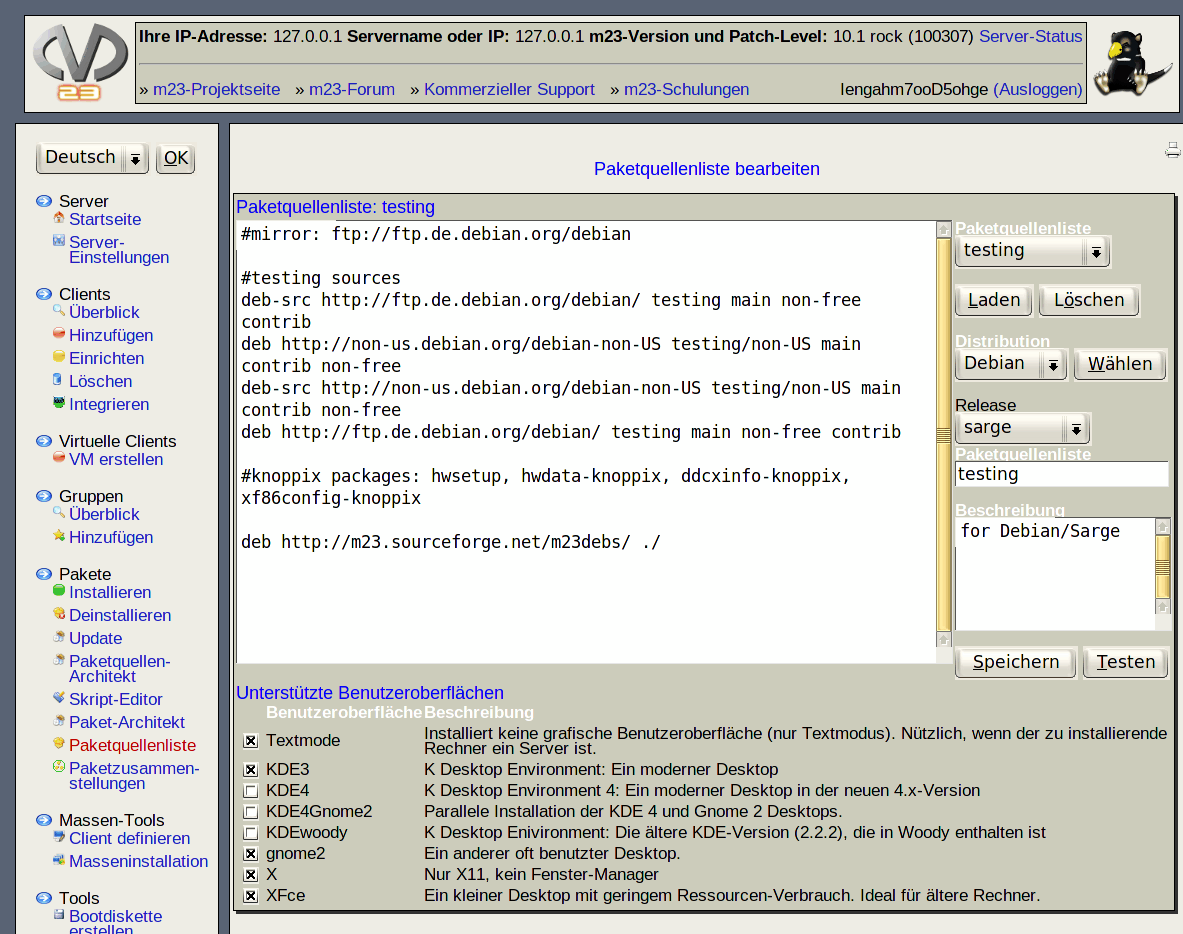
\includegraphics[scale=0.4]{/mdk/doc/manual/screenshots/de/client_sourceslist.png} \\
Softwarepakete k�nnen von verschiedenen Quellen (HTTP,FTP,CDRom, etc.) installiert werden. Verschiedene Quellen werden dann ben�tigt, wenn nicht alle Softwarepakete von einem Medium installiert werden k�nnen. Um Ihnen eine einfache M�glichkeit zu bieten, die Quellen zu verwalten, geben Sie diese ein, wie bei der ausgew�hlten Distribution gewohnt.\\
\begin{itemize}
	\item \textbf{Laden einer Paketquelle}: Zum Laden w�hlen Sie rechts oben aus der Liste die Paketquelle aus, die Sie laden m�chten. Nach Klicken auf \textit{"Laden"} wird diese in den Editor geladen.\\
	\item \textbf{L�schen der Paketquelle}: Um die in den Editor geladene Paketquelle zu l�schen, klicken Sie auf dem \textit{"L�schen"}-Button und stimmen im nachfolgenden Dialog dem L�schen zu.\\
	\item \textbf{Speichern der Paketquelle}: Es wird immer die in den Editor geladene Paketquelle gespeichert, unabh�ngig davon, welche rechts oben in der Auswahlliste angezeigt wird. W�hlen Sie zuerst die Distribution aus, f�r die die Paketliste gelten soll. Nach der Distributionswahl kann es geschehen, da� Sie zus�tzlich Angaben zu der Distribution machen m�ssen. W�hlen Sie zus�tzlich die Benutzeroberfl�chen aus der Liste unter dem Editor aus, die von der Paketquellenliste unterst�tzt werden. Suchen Sie einen Namen f�r die Paketliste aus und tragen Sie diesen in das Eingabefeld unter \textit{"Paketquellenname"} ein. Sollten Sie eine Paketquelle geladen haben, so wird der Name automatisch eingetragen. Wenn Sie m�chten, k�nnen Sie einen Kommentar in das Feld \textit{"Beschreibung"} eingeben. Klicken Sie anschlie�end auf \textit{"Speichern"}.\\
	\item \textbf{Paketquelle testen}: Nachdem Sie eine Paketquelle eingegeben haben, sollten Sie testen, ob alle Quellen ordnungsgem�� funktionieren. Nach einem Klick auf den \textit{"Test"}-Button wird versucht, die Paketbeschreibungen der Quellen herunterzuladen. Nach Abschlu� des Testes wird unten ein Testbericht angezeigt. Es kann durchaus mehrere Minuten dauern, bis der Testbericht erscheint. Dies ist abh�ngig von der Geschwindigkeit Ihrer Internetverbindung und der Geschwindigkeit der benutzten Quellpaket-Server.\\
	\item \textbf{Mirror angeben}: M�chten Sie einen anderen Mirror (voreingestellt ist ftp.debian.org) f�r die Installation des Basissystems verwenden, so geben Sie diesen in einer neuen Zeile der Paketquelle wie folgt an: \\
\begin{verbatim}
#mirror: [URL zu den Paketen]
\end{verbatim}
. Mit \textit{URL zu den Paketen} ist das Protokoll, der Hostname bzw. die IP und das Verzeichnis gemeint, wo die Pakete zu finden sind. Eine g�ltige Zeile k�nnte z.B. so aussehen \\
\begin{verbatim}
#mirror: http://192.168.7.14/debianCDs
\end{verbatim}
.\\
\end{itemize}
\subsection{Hinweis}
\begin{itemize}
\item Speichern Sie eine Paketquelle unter einem bereits existierenden Namen ab, so wird die alte Paketquelle mit dem Inhalt der neuen �berschrieben.\\
\item \textbf{Benutzeroberfl�chen} sind direkt an eine Paketquellenliste gebunden. D.h. wenn Sie eine bestimmte Paketquellenliste f�r einen Client benutzen, k�nnen Sie nur die Benutzeroberfl�chen verwenden, die Sie in diesem Dialog f�r die Paketquellenliste freigeschaltet haben. Sie sollten hier deshalb nur die Benutzeroberfl�chen ausw�hlen, die garantiert von den Paketquellen unterst�tzt werden.\\
\end{itemize}
